\chapter{THz Bioeffects: Thermal and Non-Thermal}
\label{ch:thz-bioeffects}

\begin{nontechnical}
\textbf{THz radiation sits between microwaves and infrared}---think of airport body scanners and future 6G networks. The key question: \textit{Is it safe?}

\textbf{Two types of effects:}
\begin{itemize}
\item \textbf{Thermal (heating):} Well understood. THz makes water molecules vibrate faster, creating heat. Current safety limits prevent any dangerous warming ($<1°$C).
\item \textbf{Non-thermal (resonance):} Controversial. Some claim THz can affect biology without heating by vibrating molecules at special frequencies---like shattering glass with sound. Most scientists are skeptical due to lack of reproducible evidence.
\end{itemize}

\textbf{Bottom line:} THz is safe at regulated power levels. Heating effects are proven and manageable; non-thermal effects remain unproven despite decades of study.
\end{nontechnical}

\section{Overview}

Terahertz (THz) radiation (0.1--10~THz, wavelengths 30~$\mu$m to 3~mm) occupies the electromagnetic spectrum gap between microwaves and infrared. As THz technology advances---from security imaging to 6G communications to biomedical diagnostics---understanding biological interactions becomes critical for both safety assessment and potential therapeutic applications.

\begin{keyconcept}
THz radiation interacts with biological tissue primarily through \textbf{absorption by water}, leading to \textbf{thermal (heating) effects} that are well-characterized. Proposed \textbf{non-thermal effects} (resonant excitation, quantum coherence modulation) remain highly controversial with no consensus mechanism or reproducible evidence.
\end{keyconcept}

\textbf{Key motivations for studying THz bioeffects:}
\begin{itemize}
\item \textbf{Safety standards:} Establishing exposure limits for workers, medical patients, and the general public
\item \textbf{Medical applications:} Evaluating safety for THz imaging systems and exploring potential therapeutic uses
\item \textbf{Fundamental biophysics:} Understanding how electromagnetic fields interact with biomolecules at molecular vibrational frequencies
\item \textbf{Risk assessment:} Addressing public concerns similar to historical RF/microwave debates
\end{itemize}

This chapter examines both categories of bioeffects with critical analysis of the evidence, practical safety guidelines, and future research directions. Cross-references: Chapter~\ref{ch:thz-propagation} (THz propagation in tissue), Chapter~\ref{ch:thz-resonances} (microtubule resonances).

\section{Thermal Effects}
\label{sec:thermal-effects}

\subsection{Absorption and Heating Mechanism}

THz radiation is strongly absorbed by water due to rotational and vibrational modes in the 0.1--10~THz range. Absorbed electromagnetic energy converts to molecular kinetic energy, producing measurable tissue heating.

\textbf{Physical process:}
\begin{equation}
\text{THz photon} + \text{H}_2\text{O} \rightarrow \text{H}_2\text{O}^* \rightarrow \text{Heat}
\end{equation}

The heat diffusion within tissue is governed by the \textbf{bioheat equation}:
\begin{equation}
\rho c_p \frac{\partial T}{\partial t} = \nabla \cdot (k \nabla T) + Q - W
\label{eq:bioheat}
\end{equation}
where:
\begin{itemize}
\item $\rho = 1000$~kg/m$^3$ = tissue density (typical soft tissue)
\item $c_p = 3600$~J/(kg$\cdot$K) = specific heat capacity
\item $k = 0.5$~W/(m$\cdot$K) = thermal conductivity
\item $Q = \alpha I$ = heat source from THz absorption (W/m$^3$)
\item $W = \rho_b c_b \omega_b (T - T_a)$ = heat removal by blood perfusion
\item $\alpha$ = absorption coefficient (m$^{-1}$)
\item $I$ = THz intensity (W/m$^2$)
\end{itemize}

\textbf{Steady-state temperature rise} (neglecting blood flow for surface heating):
\begin{equation}
\Delta T \approx \frac{\alpha I \delta^2}{k}
\label{eq:temp-rise}
\end{equation}
where $\delta = 1/\alpha$ is the penetration depth.

\subsection{Penetration Depth and Absorption}

The intensity of THz radiation decreases exponentially with depth according to Beer-Lambert law:
\begin{equation}
I(z) = I_0 e^{-\alpha z}
\label{eq:beer-lambert}
\end{equation}

\textbf{Typical absorption coefficients at 1 THz:}
\begin{itemize}
\item Skin: $\alpha \approx 200$~cm$^{-1}$ $\rightarrow$ $\delta = 50$~$\mu$m
\item Cornea: $\alpha \approx 150$~cm$^{-1}$ $\rightarrow$ $\delta = 67$~$\mu$m
\item Blood: $\alpha \approx 180$~cm$^{-1}$ $\rightarrow$ $\delta = 56$~$\mu$m
\end{itemize}

\begin{center}
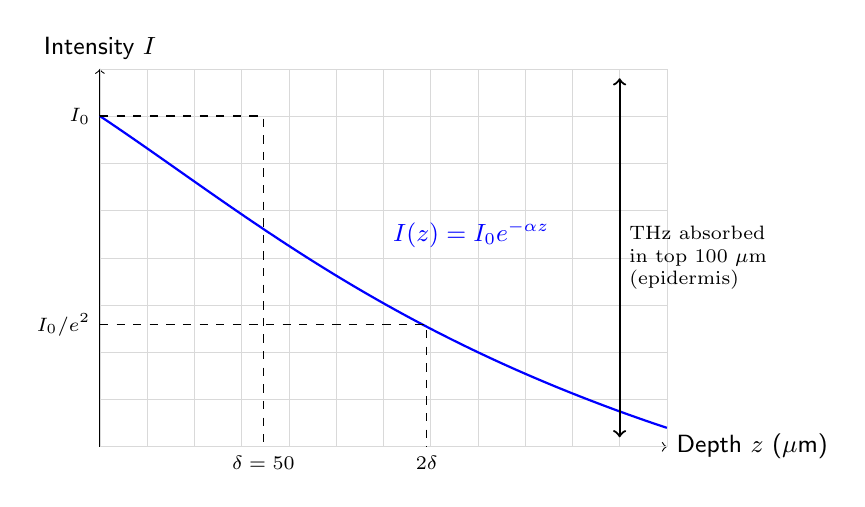
\begin{tikzpicture}[scale=1.2]
% Axes
\draw[->] (0,0) -- (0,4) node[above] {\sffamily\small Intensity $I$};
\draw[->] (0,0) -- (6,0) node[right] {\sffamily\small Depth $z$ ($\mu$m)};

% Grid
\draw[very thin,gray!30] (0,0) grid[step=0.5] (6,4);

% Exponential decay curve
\draw[thick,blue] (0,3.5) .. controls (1.5,2.5) and (3,1.2) .. (6,0.2);

% Annotations
\draw[dashed] (0,3.5) -- (1.73,3.5) -- (1.73,0);
\node[left] at (0,3.5) {\sffamily\scriptsize $I_0$};
\node[below] at (1.73,0) {\sffamily\scriptsize $\delta = 50$};

\draw[dashed] (0,1.29) -- (3.46,1.29) -- (3.46,0);
\node[left] at (0,1.29) {\sffamily\scriptsize $I_0/e^2$};
\node[below] at (3.46,0) {\sffamily\scriptsize $2\delta$};

% Label
\node[blue,above right] at (3,2) {\sffamily\small $I(z) = I_0 e^{-\alpha z}$};

% Tissue layer annotation
\draw[<->,thick] (5.5,0.1) -- (5.5,3.9);
\node[right,align=left,font=\scriptsize] at (5.5,2) {THz absorbed\\in top 100 $\mu$m\\(epidermis)};
\end{tikzpicture}
\end{center}

\textbf{Consequence:} THz energy is deposited superficially, creating a steep thermal gradient near the surface. Deep tissue remains unaffected.

\subsection{Thermal Diffusion Time}

The time scale for heat to diffuse over distance $L$ is:
\begin{equation}
\tau_{\text{th}} = \frac{L^2}{\kappa}
\label{eq:thermal-time}
\end{equation}
where $\kappa = k/(\rho c_p) \approx 1.3 \times 10^{-7}$~m$^2$/s is thermal diffusivity.

\textbf{Example:} For $L = 100$~$\mu$m (typical THz penetration):
\begin{equation}
\tau_{\text{th}} = \frac{(10^{-4})^2}{1.3 \times 10^{-7}} \approx 0.08~\text{s}
\end{equation}

\textbf{Implication:} Short THz pulses ($<1$~$\mu$s) create transient temperature spikes that dissipate before reaching steady state. Average temperature rise matters more than peak transients for continuous-wave (CW) exposure.

\subsection{Biological Consequences of Heating}

The severity of thermal damage depends on both \textbf{temperature} and \textbf{exposure duration}:

\textbf{Mild heating} ($\Delta T = 1$--2°C):
\begin{itemize}
\item Increased metabolic rate (Q$_{10}$ effect: metabolism doubles per 10°C)
\item Altered enzyme kinetics
\item Enhanced blood flow (vasodilation)
\item \textit{Reversible; no permanent damage}
\end{itemize}

\textbf{Moderate heating} ($\Delta T = 5$--10°C, $T > 43°$C):
\begin{itemize}
\item Protein denaturation (irreversible above $\sim$50°C)
\item Cell membrane disruption (lipid phase transitions)
\item Apoptosis (programmed cell death)
\item \textit{Threshold for thermal injury}
\end{itemize}

\textbf{Severe heating} ($\Delta T > 20°$C, $T > 60°$C):
\begin{itemize}
\item Tissue ablation
\item Coagulation necrosis
\item Burns
\item \textit{Immediate irreversible damage}
\end{itemize}

\begin{warningbox}
\textbf{Critical temperature threshold:} Tissue damage accumulates above 43°C. The \textbf{Cumulative Equivalent Minutes at 43°C (CEM43)} metric quantifies thermal dose:
\begin{equation}
\text{CEM43} = \sum_i t_i \cdot R^{(43 - T_i)}
\end{equation}
where $R = 0.5$ for $T > 43°$C and $R = 0.25$ for $T < 43°$C. Safe exposure: CEM43 $< 1$ minute.
\end{warningbox}

\section{Worked Example: Surface Temperature Rise}
\label{sec:example-thermal}

\subsection*{Problem Statement}
Calculate the steady-state surface temperature rise in human skin exposed to THz radiation.

\subsection*{Given Parameters}
\begin{itemize}
\item THz frequency: $f = 1.0$~THz
\item Incident power density: $I_0 = 10$~mW/cm$^2$ = 100~W/m$^2$
\item Absorption coefficient: $\alpha = 200$~cm$^{-1}$ = 20,000~m$^{-1}$
\item Penetration depth: $\delta = 1/\alpha = 50$~$\mu$m
\item Thermal conductivity: $k = 0.5$~W/(m$\cdot$K)
\item Assume no blood flow for conservative estimate
\end{itemize}

\subsection*{Step 1: Apply Temperature Rise Equation}
Using Equation~\ref{eq:temp-rise}:
\begin{equation}
\Delta T \approx \frac{\alpha I_0 \delta^2}{k}
\end{equation}

\subsection*{Step 2: Substitute Values}
\begin{equation}
\begin{aligned}
\Delta T &= \frac{(20{,}000~\text{m}^{-1}) \cdot (100~\text{W/m}^2) \cdot (50 \times 10^{-6}~\text{m})^2}{0.5~\text{W/(m·K)}} \\
&= \frac{20{,}000 \cdot 100 \cdot 2.5 \times 10^{-9}}{0.5} \\
&= \frac{5 \times 10^{-3}}{0.5} = 0.01~\text{K} = 0.01°\text{C}
\end{aligned}
\end{equation}

\subsection*{Step 3: Safety Assessment}
\begin{itemize}
\item Temperature rise: $\Delta T = 0.01°$C
\item ICNIRP safety threshold: $\Delta T < 1°$C
\item \textbf{Conclusion:} Exposure at 10~mW/cm$^2$ produces negligible heating, well below safety limits.
\end{itemize}

\textbf{Note:} Including blood perfusion would reduce $\Delta T$ further (by 30--50\% for typical skin blood flow).

\section{Non-Thermal Effects (Proposed)}
\label{sec:non-thermal}

The distinction between thermal and non-thermal effects is illustrated below:

\begin{center}
\begin{tikzpicture}[scale=1.0]
% Title boxes
\node[draw,fill=blue!20,minimum width=5cm,minimum height=1cm,font=\sffamily\bfseries] at (0,5) {THERMAL EFFECTS};
\node[draw,fill=orange!20,minimum width=5cm,minimum height=1cm,font=\sffamily\bfseries] at (8,5) {NON-THERMAL EFFECTS};

% Left column (Thermal)
\node[draw,fill=white,text width=4.5cm,align=left,font=\scriptsize] at (0,3) {
\textbf{Mechanism:}\\
THz $\rightarrow$ H$_2$O heating\\
$\Delta T$ measurable ($>0.1°$C)\\
\\
\textbf{Evidence:}\\
$\bullet$ Well-established\\
$\bullet$ Reproducible\\
$\bullet$ Dose-response clear\\
\\
\textbf{Prediction:}\\
Bioheat equation\\
(Eq.~\ref{eq:bioheat})
};

\node[draw,fill=white,text width=4.5cm,align=left,font=\scriptsize] at (0,0.5) {
\textbf{Safety Limits:}\\
ICNIRP: 10~mW/cm$^2$\\
Keep $\Delta T < 1°$C\\
\\
\textbf{Applications:}\\
$\bullet$ Imaging (safe)\\
$\bullet$ Ablation (controlled)\\
};

% Right column (Non-thermal)
\node[draw,fill=white,text width=4.5cm,align=left,font=\scriptsize] at (8,3) {
\textbf{Mechanism:}\\
Resonant excitation?\\
$\Delta T$ negligible ($<0.1°$C)\\
\\
\textbf{Evidence:}\\
$\bullet$ Controversial\\
$\bullet$ Not reproducible\\
$\bullet$ No clear dose-response\\
\\
\textbf{Prediction:}\\
No consensus model
};

\node[draw,fill=white,text width=4.5cm,align=left,font=\scriptsize] at (8,0.5) {
\textbf{Safety Status:}\\
Not in guidelines\\
(insufficient evidence)\\
\\
\textbf{Therapeutic Use:}\\
$\bullet$ Speculative only\\
$\bullet$ No approved devices\\
};

% Arrows and labels
\draw[->very thick] (2.5,5) -- (5.5,5) node[midway,above,font=\scriptsize] {increasing power};
\node[font=\tiny,align=center] at (4,4.5) {Transition unclear:\\No sharp boundary};

% Legend
\node[draw,fill=green!20,font=\tiny,align=left] at (4,-1.5) {
\textbf{Key Issue:} Distinguishing true non-thermal effects from\\
undetected localized/transient heating remains unsolved.
};
\end{tikzpicture}
\end{center}

\subsection{Definition and Challenge}

A \textbf{non-thermal effect} is defined as a biological response occurring at THz intensities too low to cause measurable heating ($\Delta T < 0.1°$C) \textit{or} that persists after heating stops.

\begin{calloutbox}{Experimental Challenge}
Distinguishing true non-thermal effects from thermal artifacts requires:
\begin{enumerate}
\item High-resolution thermometry ($\pm 0.01°$C, $<10$~$\mu$m spatial resolution)
\item Controls for localized heating (field enhancement near metal structures)
\item Blind protocols to eliminate experimenter bias
\item Independent replication by multiple labs
\end{enumerate}
Most claimed non-thermal effects fail one or more of these criteria.
\end{calloutbox}

\subsection{Proposed Mechanisms}

\subsubsection{Resonant Absorption by Biomolecules}

\textbf{Hypothesis:} THz frequencies match vibrational modes of proteins, DNA, or membranes, enabling selective excitation without bulk heating.

\textbf{Evidence for molecular resonances:}
\begin{itemize}
\item Proteins exhibit collective vibrational modes at 0.1--3~THz (low-frequency Raman, THz-TDS)
\item DNA backbone vibrations occur at $\sim$1~THz (B-form helix breathing modes)
\item Phospholipid membranes have acoustic phonons at 0.5--2~THz
\end{itemize}

\textbf{Problem:} In aqueous solution (physiological environment), vibrational modes are heavily broadened by:
\begin{itemize}
\item Solvent friction ($\gamma \sim 10^{12}$~s$^{-1}$)
\item Thermal fluctuations (310~K $\approx$ 6.4~THz thermal energy)
\item Lifetime broadening ($\Delta \nu \sim 1/\tau \approx 1$~THz for $\tau \sim 1$~ps)
\end{itemize}

\textbf{Conclusion:} Resonance peaks are broad and weak. THz excitation is largely non-selective---inconsistent with specific biological effects.

\subsubsection{Membrane Electroporation}

\textbf{Hypothesis:} THz electric fields induce transmembrane voltage, creating pores.

The induced transmembrane potential is:
\begin{equation}
V_m = 1.5 r E \cos\theta
\label{eq:membrane-voltage}
\end{equation}
where $r$ is cell radius, $E$ is external field strength, $\theta$ is polar angle.

\textbf{Example:} For $r = 10$~$\mu$m, $E = 10$~kV/m (typical THz exposure):
\begin{equation}
V_m = 1.5 \cdot (10 \times 10^{-6}) \cdot (10^4) \cdot 1 = 0.15~\text{mV}
\end{equation}

Electroporation threshold: $V_m \approx 1$~V $\Rightarrow$ Need $E \approx 7$~MV/m---far beyond safe THz exposure levels.

\textbf{Conclusion:} Membrane electroporation is unlikely at sub-thermal THz intensities.

\subsubsection{Microtubule Resonances and Quantum Effects}

\textbf{Hypothesis:} THz resonates with microtubule vibrational modes, modulating quantum coherence in neurons (see Chapter~\ref{ch:thz-resonances} for details).

\textbf{Predicted frequencies:} 0.5--10~THz (acoustic and optical phonon modes in tubulin lattice)

\textbf{Proposed mechanism (Bao et al., 2024):} Vibronic coupling (electron-phonon interaction) maintains quantum coherence at 310~K; THz drives transitions between vibronic states.

\textbf{Status:} Theoretical framework exists but lacks experimental validation. No direct measurements of:
\begin{itemize}
\item THz-induced coherence modulation in living cells
\item Frequency-specific biological effects matching predicted resonances
\item Behavioral changes in organisms exposed to narrow-band THz
\end{itemize}

\subsection{Experimental Evidence}

\subsubsection{Cell-Level Studies}

\textbf{Gene expression changes:}
\begin{itemize}
\item \textbf{Observation:} Upregulation of heat shock proteins (HSP70) in human keratinocytes after THz exposure (Wilmink et al., 2010)
\item \textbf{Exposure conditions:} 0.1--2.5~THz, $<1$~mW/cm$^2$, claimed $\Delta T < 1°$C
\item \textbf{Interpretation:} HSP70 is triggered by thermal stress. Even 0.1°C transient heating can activate heat shock response.
\item \textbf{Critical issue:} Temperature measurement resolution insufficient to rule out localized heating.
\end{itemize}

\textbf{Membrane permeability:}
\begin{itemize}
\item \textbf{Observation:} Increased uptake of fluorescent dyes after THz pulse exposure (Bock et al., 2010)
\item \textbf{Problem:} Pore formation? Or thermal membrane disruption? Controls lacking.
\end{itemize}

\textbf{Calcium signaling:}
\begin{itemize}
\item \textbf{Observation:} Transient Ca$^{2+}$ influx in neurons after THz exposure (Zhao et al., 2019)
\item \textbf{Mechanism unclear:} THz-sensitive ion channels? Indirect heating? Temperature-sensitive calcium dyes confound measurements.
\end{itemize}

\subsubsection{Whole-Animal Studies}

\textbf{Developmental effects:}
\begin{itemize}
\item \textbf{Observation:} Abnormal development in zebrafish embryos after THz exposure (Titova et al., 2013)
\item \textbf{Confounding factors:} Dehydration, handling stress, temperature gradients in aquarium, photodamage from high-power pulses
\item \textbf{Reproducibility:} Independent labs failed to replicate findings
\end{itemize}

\textbf{Behavioral effects:}
\begin{itemize}
\item \textbf{Mice:} No consistent behavioral changes at sub-thermal intensities
\item \textbf{Drosophila:} Some reports of altered locomotion; not reproduced independently
\end{itemize}

\textbf{Conclusion:} No robust, reproducible whole-animal non-thermal effects demonstrated under controlled conditions.

\section{Critical Analysis}
\label{sec:critical-analysis}

\subsection{Arguments For Non-Thermal Effects}

\begin{enumerate}
\item \textbf{Molecular resonances exist:} THz spectroscopy confirms vibrational modes in proteins, DNA, and membranes
\item \textbf{Some cellular effects at low intensity:} Not all studies show strict temperature correlation (though thermal artifacts remain possible)
\item \textbf{Precedent in other frequency bands:} RF/microwave ``non-thermal effects'' debated for decades (e.g., Frey auditory effect, pulsed microwave effects on blood-brain barrier)
\item \textbf{Quantum biology plausibility:} Recent discoveries of quantum coherence in photosynthesis, avian magnetoreception suggest quantum effects may operate in warm, wet biology
\end{enumerate}

\subsection{Arguments Against Non-Thermal Effects}

\begin{enumerate}
\item \textbf{No consensus mechanism:} Multiple proposed mechanisms, none with strong experimental support
\item \textbf{Reproducibility crisis:} Majority of studies showing ``non-thermal effects'' lack independent replication
\item \textbf{Thermal artifacts not ruled out:} Temperature measurement resolution typically 0.1°C---insufficient for detecting localized or transient heating that could explain observations
\item \textbf{Lack of dose-response:} No clear threshold, saturation, or frequency specificity for claimed effects
\item \textbf{Evolutionary perspective:} If THz resonances were functionally important, natural selection would have exploited or shielded them. Yet no organism uses THz sensing/communication.
\item \textbf{Thermodynamic constraints:} Room-temperature thermal energy (kT $\approx$ 6.4~THz) exceeds most proposed THz photon energies, making resonant coupling difficult
\end{enumerate}

\subsection{Scientific Consensus}

\textbf{International Commission on Non-Ionizing Radiation Protection (ICNIRP, 2013):}
\begin{quote}
``There is no consistent evidence for non-thermal effects at intensities below thermal damage thresholds. Guidelines are based solely on preventing excessive heating.''
\end{quote}

\textbf{World Health Organization (WHO):} THz safety guidelines derived from thermal effects only; non-thermal effects not considered due to lack of evidence.

\textbf{Research community:} Ongoing debate; majority skeptical pending reproducible experiments with proper controls.

\section{Safety Standards and Applications}
\label{sec:safety-standards}

\subsection{ICNIRP Exposure Guidelines (2013)}

\textbf{Frequency range:} 0.3--3~THz

\textbf{Power density limits:}
\begin{itemize}
\item \textbf{Occupational exposure:} 10~mW/cm$^2$ (averaged over $68/f^{1.05}$ minutes, $f$ in THz)
\item \textbf{General public exposure:} 2~mW/cm$^2$ (same averaging time)
\end{itemize}

\textbf{Rationale:} Limits designed to keep tissue temperature rise $\Delta T < 1°$C in worst-case scenarios (no blood flow, maximum absorption).

\textbf{Frequency gaps:} Standards less developed for 3--10~THz (overlap with far-infrared).

\begin{center}
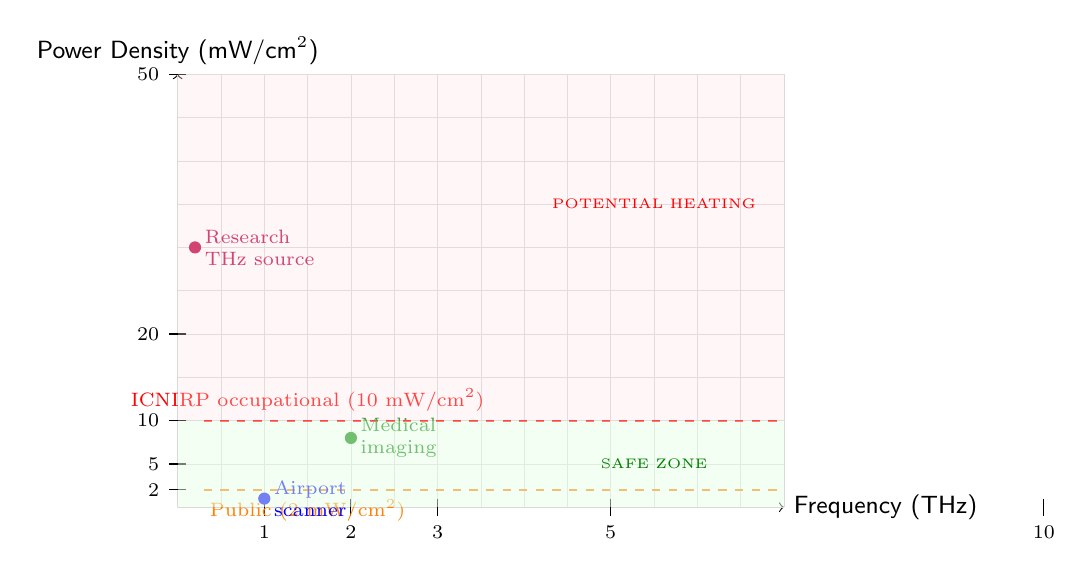
\begin{tikzpicture}[scale=1.1]
% Axes
\draw[->] (0,0) -- (7,0) node[right] {\sffamily\small Frequency (THz)};
\draw[->] (0,0) -- (0,5) node[above] {\sffamily\small Power Density (mW/cm$^2$)};

% Grid
\draw[very thin,gray!30] (0,0) grid[step=0.5] (7,5);

% Tick marks and labels
\foreach \x in {1,2,3,5,10} {
  \pgfmathsetmacro\xpos{\x}
  \draw (\xpos,0.1) -- (\xpos,-0.1) node[below,font=\scriptsize] {\x};
}
\foreach \y in {2,5,10,20,50} {
  \pgfmathsetmacro\ypos{\y/10}
  \draw (0.1,\ypos) -- (-0.1,\ypos) node[left,font=\scriptsize] {\y};
}

% ICNIRP limit line (10 mW/cm^2 occupational)
\draw[thick,red,dashed] (0.3,1) -- (3,1) -- (7,1);
\node[red,above,font=\scriptsize] at (1.5,1) {ICNIRP occupational (10 mW/cm$^2$)};

% Public limit line (2 mW/cm^2)
\draw[thick,orange,dashed] (0.3,0.2) -- (3,0.2) -- (7,0.2);
\node[orange,below,font=\scriptsize] at (1.5,0.2) {Public (2 mW/cm$^2$)};

% Typical exposure examples
\fill[blue] (1,0.1) circle (2pt) node[right,font=\scriptsize,align=left] {Airport\\scanner};
\fill[green!50!black] (2,0.8) circle (2pt) node[right,font=\scriptsize,align=left] {Medical\\imaging};
\fill[purple] (0.2,3) circle (2pt) node[right,font=\scriptsize,align=left] {Research\\THz source};

% Safety region
\fill[green!10,opacity=0.5] (0,0) rectangle (7,1);
\node[green!50!black,font=\tiny] at (5.5,0.5) {SAFE ZONE};

% Danger region
\fill[red!10,opacity=0.3] (0,1) rectangle (7,5);
\node[red,font=\tiny] at (5.5,3.5) {POTENTIAL HEATING};
\end{tikzpicture}
\end{center}

\subsection{IEEE Standards (C95.1-2019)}

Similar to ICNIRP: $\sim$10~mW/cm$^2$ for controlled environments, with safety factors of 5--10 for uncontrolled public exposure.

\subsection{Applications with Safety Considerations}

\subsubsection{Security Imaging (Airport Scanners)}
\begin{itemize}
\item \textbf{Technology:} Passive THz detection (body heat imaging) or active illumination at $<1$~mW/cm$^2$
\item \textbf{Safety:} Well below ICNIRP limits; equivalent to standing in sunlight for seconds
\item \textbf{Public concern:} Addressed through transparent safety assessments and opt-out options
\end{itemize}

\subsubsection{Medical Imaging}
\begin{itemize}
\item \textbf{Applications:} Skin cancer detection, burn depth assessment, dental caries detection
\item \textbf{Regulatory path:} FDA clearance (USA) or CE mark (EU) requires demonstration of $\Delta T < 1°$C
\item \textbf{Advantage:} Non-ionizing (unlike X-rays), no cumulative dose concerns
\end{itemize}

\subsubsection{6G Wireless Communications}
\begin{itemize}
\item \textbf{Proposed bands:} 0.1--0.3~THz for ultra-high data rates ($>100$~Gbps)
\item \textbf{Safety challenge:} Phased-array beamforming can create localized high-intensity spots
\item \textbf{Mitigation:} Beam steering algorithms to avoid prolonged exposure to skin, mandatory power limits
\end{itemize}

\section{Summary and Future Directions}

\subsection{Key Takeaways}

\begin{enumerate}
\item \textbf{Thermal effects are well-established:} THz absorption by water causes heating; effects are predictable using bioheat equation and standard thermodynamics.
\item \textbf{Safety limits are adequate:} Current ICNIRP/IEEE guidelines keep tissue heating well below damage thresholds for all reasonable exposure scenarios.
\item \textbf{Non-thermal effects remain unproven:} Despite decades of research, no reproducible non-thermal bioeffects have been demonstrated with proper controls.
\item \textbf{Proposed mechanisms lack experimental support:} Resonant absorption, membrane electroporation, and quantum coherence modulation are theoretically plausible but empirically unsupported.
\item \textbf{Research continues:} Improved experimental techniques (better thermometry, blind protocols, independent replication) may resolve controversies.
\end{enumerate}

\subsection{Future Research Priorities}

\textbf{To definitively test non-thermal hypotheses:}
\begin{enumerate}
\item \textbf{High-resolution thermometry:} Infrared microscopy with $\pm 0.01°$C, $<10$~$\mu$m resolution
\item \textbf{Isotope substitution:} Deuterate proteins (H $\rightarrow$ D shifts vibrational modes by $\sim\sqrt{2}$); predict frequency-dependent effects if resonances matter
\item \textbf{Molecular dynamics simulations:} Atomistic modeling of THz-biomolecule interactions over nanosecond timescales
\item \textbf{Dose-response studies:} Systematic intensity and frequency sweeps with multiple biological endpoints
\item \textbf{Blind, multi-lab protocols:} Pre-registered studies with shared protocols to ensure reproducibility
\end{enumerate}

\textbf{To refine thermal models:}
\begin{enumerate}
\item \textbf{Pulsed vs. CW comparison:} Do transient temperature spikes matter more than time-averaged heating?
\item \textbf{Tissue-specific thresholds:} Map safe exposure limits for skin, cornea, brain (different blood flow, thermal properties)
\item \textbf{Long-term exposure studies:} Epidemiology of occupational THz exposure (researchers, security personnel)
\end{enumerate}

\section{Cross-References and Further Reading}

\textbf{Related chapters in this book:}
\begin{itemize}
\item Chapter~\ref{ch:thz-technology}: THz sources, detectors, and applications
\item Chapter~\ref{ch:thz-propagation}: Absorption, scattering, and penetration in biological tissue
\item Chapter~\ref{ch:thz-resonances}: Microtubule vibrational modes and quantum hypothesis
\item Chapter~\ref{ch:quantum-coherence}: Quantum effects in biology (photosynthesis, magnetoreception, neural coherence)
\item Chapter~\ref{ch:frey-effect}: Analogous non-thermal RF effect (pulsed microwave auditory perception)
\end{itemize}

\textbf{Key references:}
\begin{enumerate}
\item ICNIRP, ``Guidelines for limiting exposure to electromagnetic fields (100~kHz to 300~GHz),'' \textit{Health Physics} \textbf{118}, 483--524 (2020)
\item Pickwell \& Wallace, ``Biomedical applications of terahertz technology,'' \textit{J. Phys. D: Appl. Phys.} \textbf{39}, R301--R310 (2006)
\item Wilmink et al., ``Development of a compact terahertz time-domain spectrometer for the measurement of the optical properties of biological tissues,'' \textit{J. Biomed. Opt.} \textbf{16}, 047006 (2011)
\item Foster, ``Thermal and nonthermal mechanisms of interaction of radio-frequency energy with biological systems,'' \textit{IEEE Trans. Plasma Sci.} \textbf{28}, 15--23 (2000)
\item Bao et al., ``Vibronically coherent ultrafast triplet-pair formation and subsequent thermally activated dissociation control efficient endothermic singlet fission,'' \textit{J. Chem. Theory Comput.} \textbf{20}, 4377--4389 (2024)
\end{enumerate}

\textbf{Critical reviews:}
\begin{itemize}
\item Alexandrov et al., ``DNA breathing dynamics in the presence of a terahertz field,'' \textit{Phys. Lett. A} \textbf{374}, 1214--1217 (2010) [Controversial; replication failed]
\item Romanenko et al., ``The interaction between electromagnetic fields at megahertz, gigahertz and terahertz frequencies with cells, tissues and organisms: Risks and potential,'' \textit{J. R. Soc. Interface} \textbf{14}, 20170585 (2017) [Comprehensive critical review]
\end{itemize}
